\documentclass[a4paper,12pt]{article}

\usepackage{graphicx} % Required for inserting images
\usepackage{amsmath,amssymb,amsfonts}
\usepackage{subcaption}
% -----------------------
% Package Imports
% -----------------------

% Set page margins
\usepackage[a4paper, top=1in, bottom=0.8in, left=1.1in, right=0.8in]{geometry}

% Use Times New Roman font
\usepackage{times}

% Add page numbering
\pagestyle{plain}
\usepackage{multirow}
% Enable graphics inclusion
\usepackage{graphicx}
\usepackage{float}
% Enable code listings
\usepackage{listings}
\usepackage{xcolor} % For customizing code colors

% Define MATLAB style for listings
\lstdefinestyle{vscode-light}{
	language=Matlab,
	basicstyle=\ttfamily\footnotesize,
	keywordstyle=\color{blue},
	commentstyle=\color{gray},
	stringstyle=\color{red},
	numberstyle=\tiny\color{black},
	numbersep=5pt,
	frame=single,
	backgroundcolor=\color{white!10},
	breaklines=true,
	captionpos=b,
	tabsize=4,
	showstringspaces=false,
	numbers=left,  % Enable line numbering on the left
	stepnumber=1,  % Line numbers increment by 1
	numberfirstline=true, % Number the first line
}
\setlength{\parindent}{0pt}


\begin{document}
	\section{Experiment No. 2}
	
	\section{Experiment Title }
	Observation \& Verification of Amplitude Modulation \& Demodulation
	\section{Objective}
	
	The objectives of this lab are as follows:
	\begin{itemize}
		\item To explore the practical implementation and circuit configurations of modulation and
		demodulation kits
		\item To understand the working principles of modulation and demodulation techniques
		
	\end{itemize}
	
	\section{Theory}


\subsection{Amplitude Modulation}
In AM, the amplitude of the carrier signal is modulated by the message signal, while the frequency and phase of the carrier remain constant. Let’s define the key signals involved:

\begin{enumerate}
	\item \textbf{Message Signal}: The information signal to be transmitted, denoted as \( m(t) \). Typically, it is a low-frequency signal, e.g., an audio signal.
	\item \textbf{Carrier Signal}: A high-frequency sinusoidal signal, denoted as \( c(t) = A_c \cos(2\pi f_c t) \), where \( A_c \) is the carrier amplitude and \( f_c \) is the carrier frequency.
	\item \textbf{Modulated Signal}: The resulting AM signal, denoted as \( s(t) \).
\end{enumerate}

\subsection{Modulation Process}
The AM signal is generated by multiplying the carrier signal by a term that includes the message signal. The general expression for the AM signal is:

\begin{equation}
	s(t) = \left[ A_c + m(t) \right] \cos(2\pi f_c t)
\end{equation}

To normalize the modulation, the message signal is often scaled by the modulation index \( m \), defined as:

\begin{equation}
	m = \frac{A_m}{A_c}
\end{equation}

where \( A_m \) is the peak amplitude of the message signal \( m(t) \). Assuming \( m(t) = A_m \cos(2\pi f_m t) \), where \( f_m \) is the message signal frequency, the AM signal becomes:

\begin{equation}
	s(t) = A_c \left[ 1 + m \cos(2\pi f_m t) \right] \cos(2\pi f_c t)
\end{equation}

Expanding this using the trigonometric identity \( \cos A \cos B = \frac{1}{2} [\cos(A+B) + \cos(A-B)] \), we get:

\begin{equation}
	s(t) = A_c \cos(2\pi f_c t) + \frac{m A_c}{2} \cos[2\pi (f_c + f_m) t] + \frac{m A_c}{2} \cos[2\pi (f_c - f_m) t]
\end{equation}

This shows that the AM signal consists of:
\begin{itemize}
	\item The carrier component at frequency \( f_c \).
	\item The upper side-band at \( f_c + f_m \).
	\item The lower side-band at \( f_c - f_m \).
\end{itemize}

\subsection{Modulation Index}
The modulation index \( m \) determines the extent of modulation:
\begin{enumerate}
	\item \textbf{Under-modulation} (\( m < 1 \)): The envelope of the AM signal follows the message signal without distortion.
	\item \textbf{Full modulation} (\( m = 1 \)): The carrier amplitude varies between 0 and \( 2A_c \), maximizing the side-band power without distortion.
	\item \textbf{Over-modulation} (\( m > 1 \)): The envelope becomes distorted, leading to signal clipping and recovery challenges during demodulation.
\end{enumerate}

\subsection{Amplitude Demodulation}
Demodulation is the process of extracting the original message signal \( m(t) \) from the AM signal \( s(t) \). The most common method is \textbf{envelope detection}, which is simple and effective for standard AM signals.
\begin{figure}[H]
	\centering
	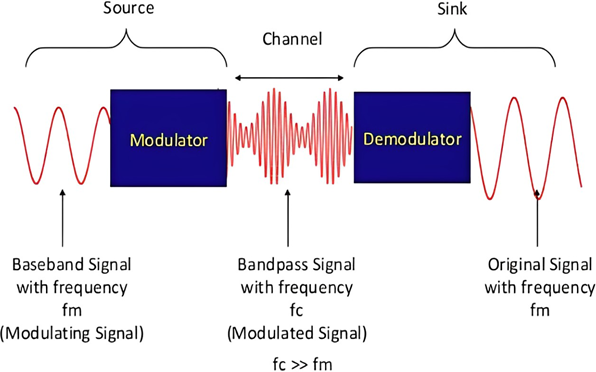
\includegraphics[width=0.7\linewidth]{Images/screenshot001}
	\caption{Demodulation process}
	\label{fig:screenshot001}
\end{figure}
\subsection{Envelope Detection}
The AM signal \( s(t) = A_c \left[ 1 + m \cos(2\pi f_m t) \right] \cos(2\pi f_c t) \) has an envelope given by \\ \( A_c \left| 1 + m \cos(2\pi f_m t) \right| \). The steps for envelope detection are:

\begin{enumerate}
	\item \textbf{Rectification}: Pass the AM signal through a diode to obtain the positive portion, yielding \( |s(t)| \).
	\item \textbf{Low-pass filtering}: Apply a low-pass filter to remove the high-frequency carrier components, leaving the envelope \( A_c \left[ 1 + m \cos(2\pi f_m t) \right] \).
	\item \textbf{DC removal}: Subtract the DC component \( A_c \) (using a capacitor or high-pass filter) to recover \( m(t) \).
\end{enumerate}

Mathematically, the output of the envelope detector, after filtering, is proportional to:

\begin{equation}
	m(t) = A_m \cos(2\pi f_m t)
\end{equation}

\subsection{Conditions for Successful Demodulation}
For envelope detection to work effectively:
\begin{enumerate}
	\item The modulation index should satisfy \( m \leq 1 \) to avoid distortion due to over-modulation.
	\item The carrier frequency \( f_c \) must be much higher than the message frequency \( f_m \) (\( f_c \gg f_m \)) to ensure the envelope can be accurately tracked.
\end{enumerate}

\subsection{Required Apparatus}
	\begin{enumerate}

	\item	Amplitude modulation transmitter kit.
	\item	Amplitude Demodulator Receiver kit.
	\item Connecting wires.
\end{enumerate}

\newpage
\subsubsection{MATLAB Code:}
\begin{lstlisting}[style=vscode-light, caption={Solving Non-linear Equation Using Newton-Raphson Method in MATLAB.} ]
	% MATLAB code for AM modulation with separate plots
	% Message and carrier signals, and AM signals for under, full, and over modulation
	clear all;
	close all;
	% Parameters
	t = 0:0.0001:0.1; % Time vector (0 to 0.1s, 10001 samples)
	fm = 50; % Message signal frequency (50 Hz)
	fc = 500; % Carrier signal frequency (500 Hz)
	Am = 1; % Message signal amplitude
	Ac = 1; % Carrier signal amplitude
	
	% Message and carrier signals
	m_t = Am * cos(2 * pi * fm * t); % Message signal
	c_t = Ac * cos(2 * pi * fc * t); % Carrier signal
	
	% Modulation indices for under, full, and over modulation
	m_indices = [0.5, 1, 1.5]; % m = 0.5 (under), 1 (full), 1.5 (over)
	
	% Plot 1: Message Signal
	figure('Position', [100, 100, 600, 400]);
	plot(t, m_t, 'b', 'LineWidth', 1.5);
	title('Message Signal');
	xlabel('Time (s)');
	ylabel('Amplitude');
	grid on;
	set(gcf, 'Color', 'w');
	
	% Plot 2: Carrier Signal
	figure('Position', [750, 100, 600, 400]);
	plot(t, c_t, 'r', 'LineWidth', 1.5);
	title('Carrier Signal');
	xlabel('Time (s)');
	ylabel('Amplitude');
	grid on;
	set(gcf, 'Color', 'w');
	
	% Plot AM signals for different modulation indices
	for i = 1:length(m_indices)
	m = m_indices(i);
	s_t = (1 + m * m_t / Am) .* c_t; % AM signal: s(t) = [1 + m*m(t)/Am]*c(t)
	
	% Create a new figure for each AM signal
	figure('Position', [100 + (i-1)*650, 600, 600, 400]);
	plot(t, s_t, 'k', 'LineWidth', 1.5);
	title(['AM Signal (m = ', num2str(m), ')']);
	xlabel('Time (s)');
	ylabel('Amplitude');
	grid on;
	set(gcf, 'Color', 'w');
	end
	
	
	
\end{lstlisting}
\section{Plot Diagram}
\begin{figure}[H]
	\centering
	\begin{subfigure}[t]{0.49\textwidth}
		\centering
		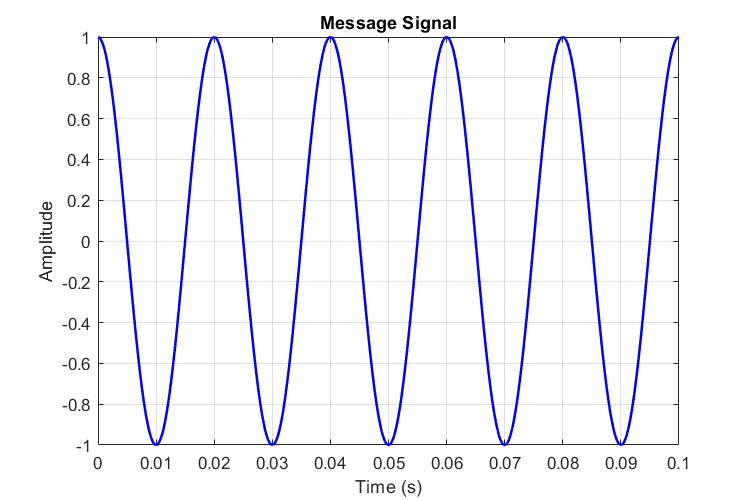
\includegraphics[width=1\linewidth]{Images/1.1}
		\caption{Message Signal}
		\vspace{0.1cm}
	\end{subfigure}
	\hfil
	\begin{subfigure}[t]{0.49\textwidth}
		\centering
		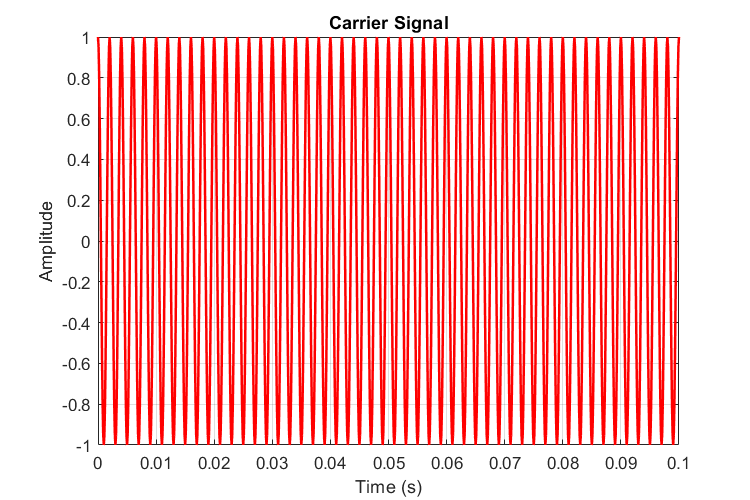
\includegraphics[width=1\linewidth]{Images/2.2}
		\caption{ Carrier Signal}
	\end{subfigure}
	
	\begin{subfigure}[t]{0.49\textwidth}
		\centering
		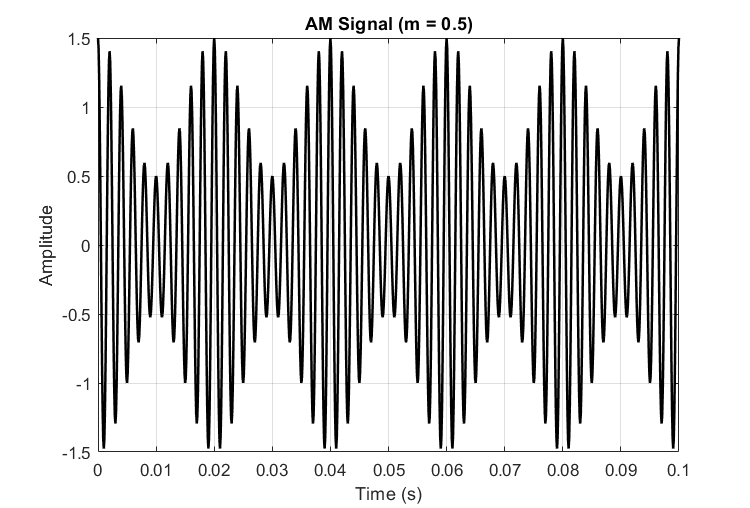
\includegraphics[width=1\linewidth]{Images/3.3}
		\caption{ modulation index , m=0.5}
	\end{subfigure}
	\hfil
	\begin{subfigure}[t]{0.49\textwidth}
		\centering
		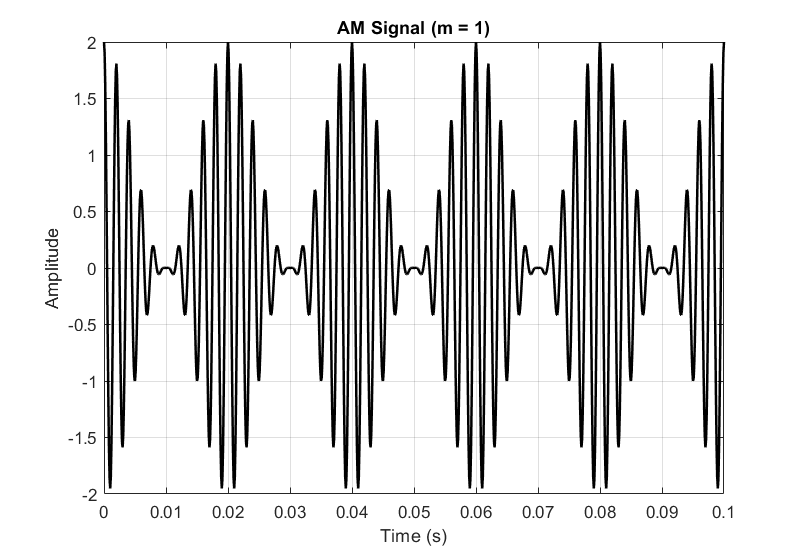
\includegraphics[width=1\linewidth]{Images/4.4}
		\caption{modulation index , m=1}
	\end{subfigure}
	
	\begin{subfigure}[t]{0.55\textwidth}
		\centering
		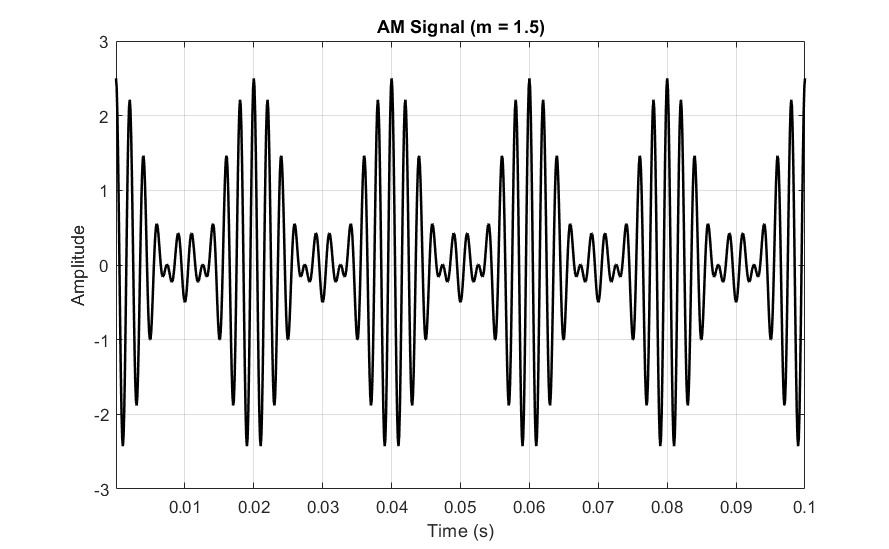
\includegraphics[width=1\linewidth]{Images/5.5}
		\caption{ modulation index , m=1.5}
	\end{subfigure}
\end{figure}

\newpage
	\section{Experimental Setup}
\begin{figure}[H]
	\centering
	\begin{subfigure}[t]{1\textwidth}
		\centering
		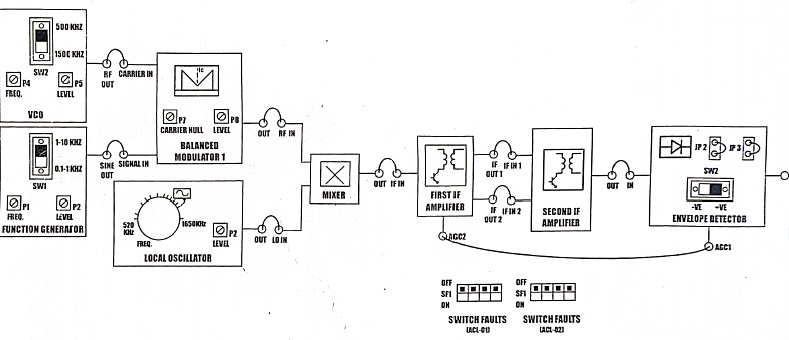
\includegraphics[width=1\linewidth]{Images/7}
		\caption{ Required circuit diagram }
		\vspace{2cm}
	\end{subfigure}
	
	\begin{subfigure}[t]{1\textwidth}
		\centering
		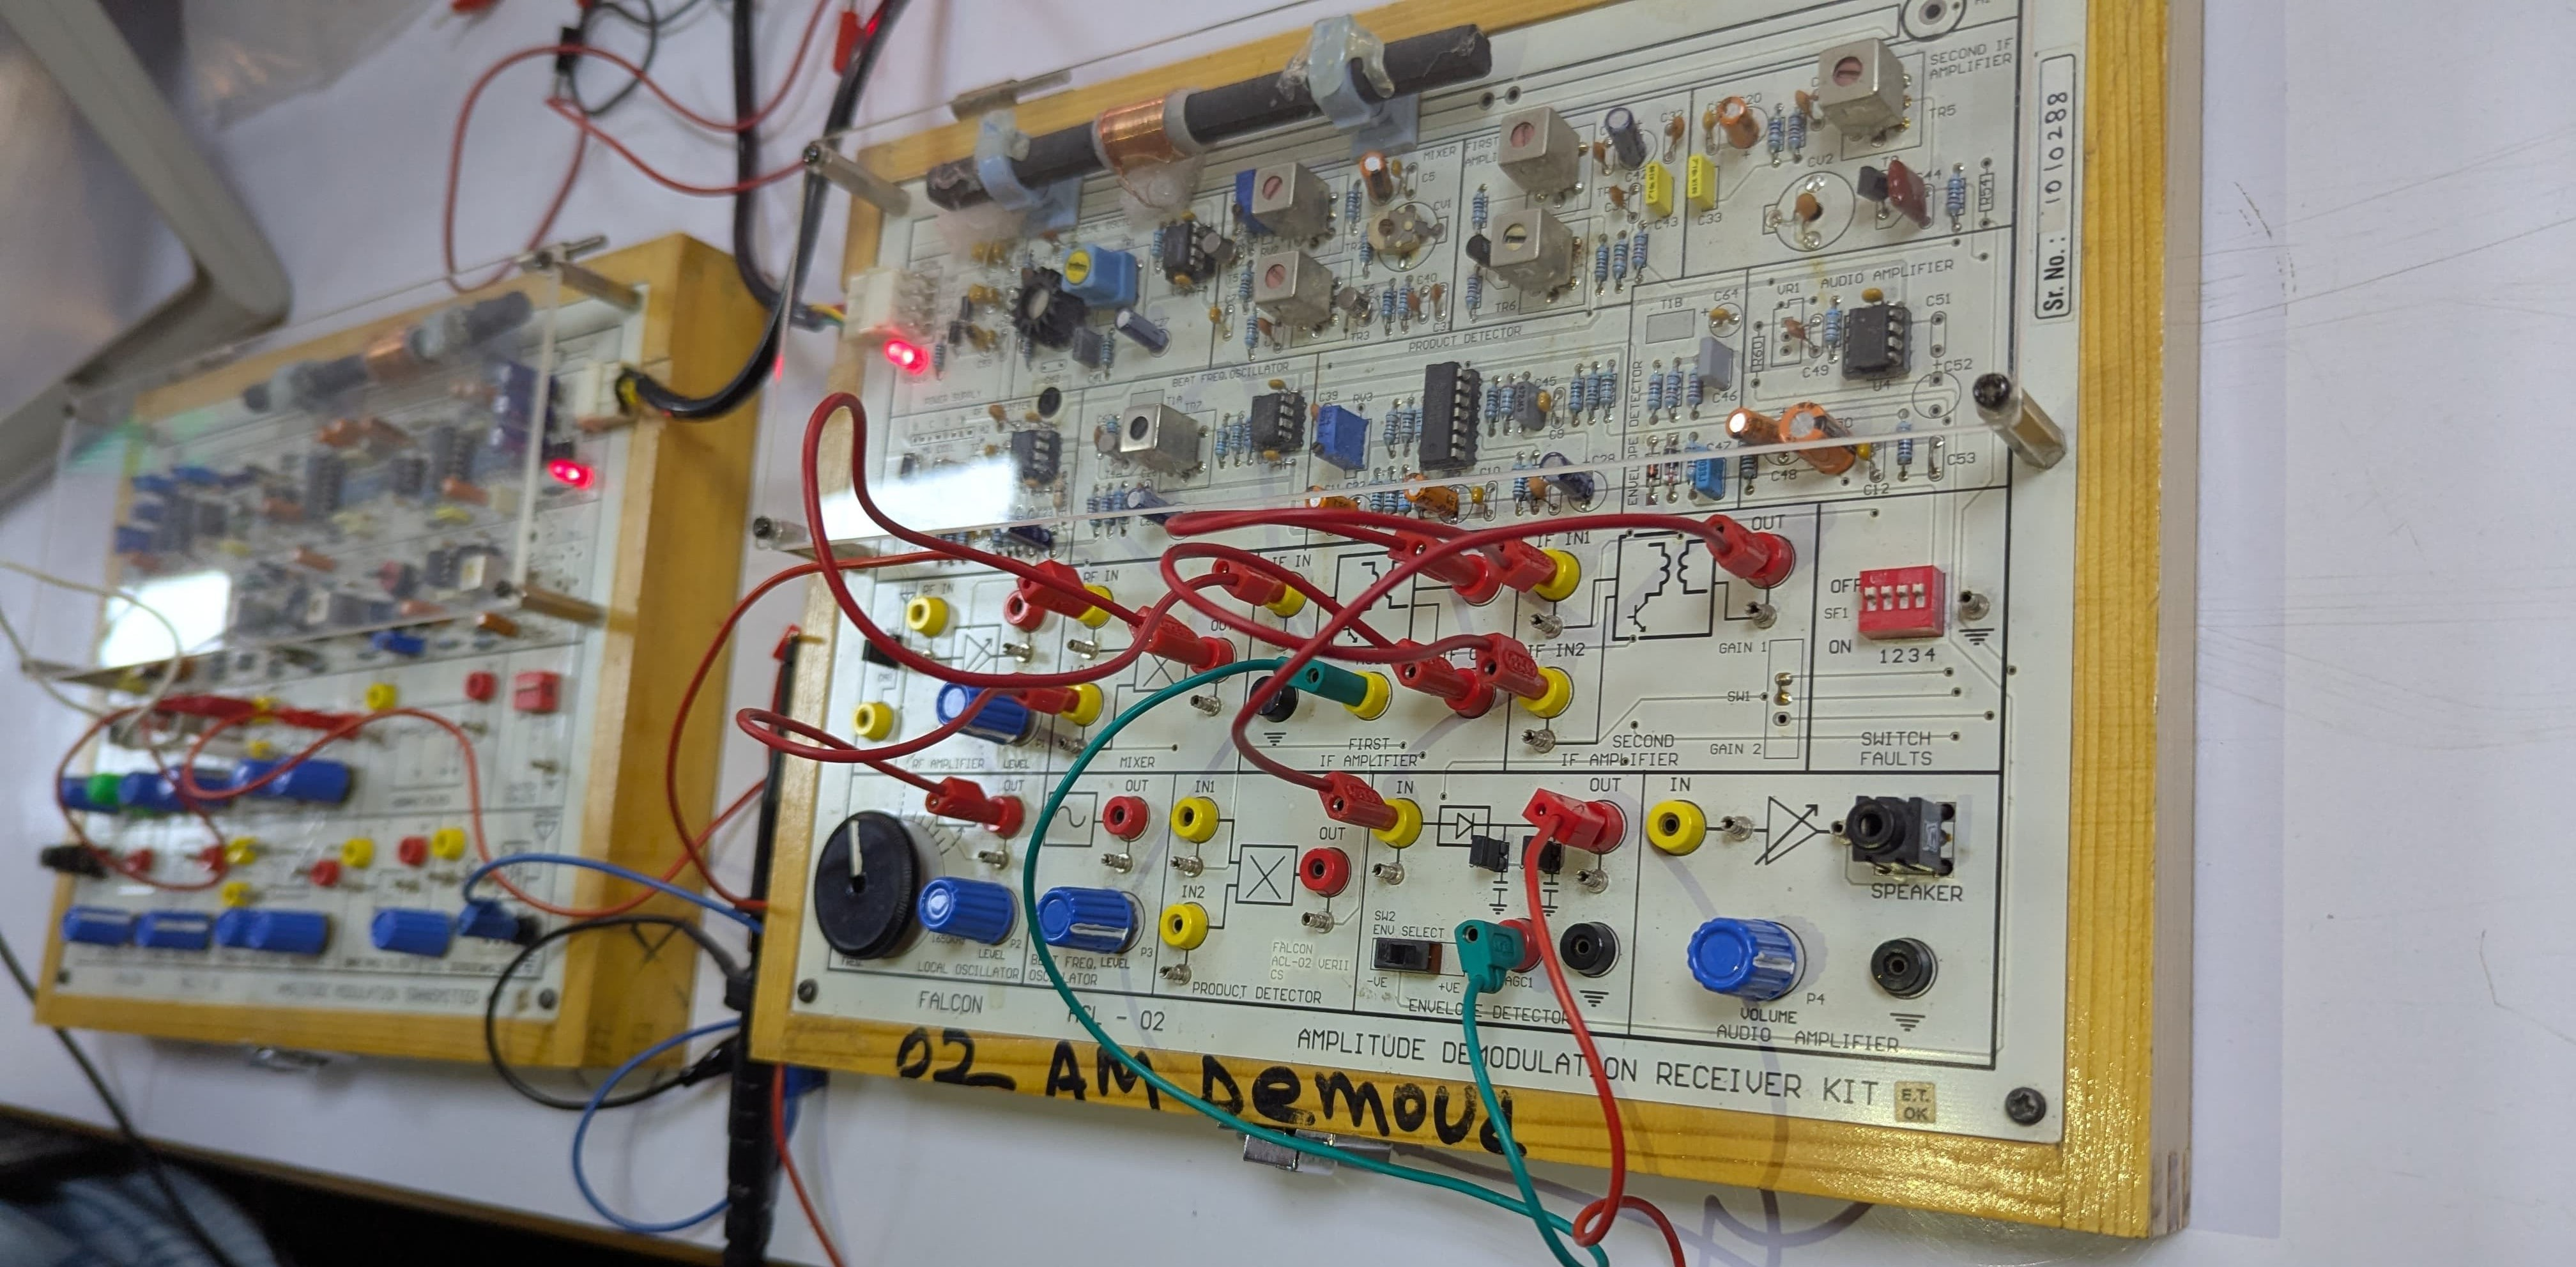
\includegraphics[width=0.95\linewidth]{Images/01}
		\caption{ Actual setup}
	\end{subfigure}
\end{figure}
\newpage
\section{Experimental Wavehape}
	\begin{figure}[H]
	\centering
	\includegraphics[width=.65\linewidth, height=0.26\textheight]{"Images/1"}
	\caption{Message Signal}
    \end{figure}
    
    	\begin{figure}[H]
    	\centering
    	\includegraphics[width=.65\linewidth, height=0.26\textheight]{"Images/2"}
    	\caption{Carrier Signal}
    \end{figure}
    
    	\begin{figure}[H]
    	\centering
    	\includegraphics[width=.65\linewidth, height=0.26\textheight]{"Images/3"}
    	\caption{modulation index , m $=$ 1}
    \end{figure}
    
    	\begin{figure}[H]
    	\centering
    	\includegraphics[width=.65\linewidth, height=0.26\textheight]{"Images/4"}
    	\caption{modulation index , m $<$ 1}
    \end{figure}
    
    	\begin{figure}[H]
    	\centering
    	\includegraphics[width=.65\linewidth, height=0.26\textheight]{"Images/5"}
    	\caption{modulation index , m $>$ 1}
    \end{figure}
    
    	\begin{figure}[H]
    	\centering
    	\includegraphics[width=.65\linewidth, height=0.26\textheight]{"Images/6"}
    	\caption{Demodulated Signal}
    \end{figure}
    \section{Discussion}
  In the experiment, amplitude modulation and demodulation were observed using an amplitude‐modulation transmitter kit and an amplitude‐demodulation receiver kit. The transmitter circuit was assembled according to the manual, and both the message and carrier signals were generated. These two signals were combined to produce the modulated waveform. The modulated signal was then fed into the Demodulator kit, and the desired message signal was recovered at the output by use of the envelope detector.
  
    \newpage
    	
\end{document}
